% Options for packages loaded elsewhere
\PassOptionsToPackage{unicode}{hyperref}
\PassOptionsToPackage{hyphens}{url}
%
\documentclass[
]{article}
\usepackage{amsmath,amssymb}
\usepackage{iftex}
\ifPDFTeX
  \usepackage[T1]{fontenc}
  \usepackage[utf8]{inputenc}
  \usepackage{textcomp} % provide euro and other symbols
\else % if luatex or xetex
  \usepackage{unicode-math} % this also loads fontspec
  \defaultfontfeatures{Scale=MatchLowercase}
  \defaultfontfeatures[\rmfamily]{Ligatures=TeX,Scale=1}
\fi
\usepackage{lmodern}
\ifPDFTeX\else
  % xetex/luatex font selection
\fi
% Use upquote if available, for straight quotes in verbatim environments
\IfFileExists{upquote.sty}{\usepackage{upquote}}{}
\IfFileExists{microtype.sty}{% use microtype if available
  \usepackage[]{microtype}
  \UseMicrotypeSet[protrusion]{basicmath} % disable protrusion for tt fonts
}{}
\makeatletter
\@ifundefined{KOMAClassName}{% if non-KOMA class
  \IfFileExists{parskip.sty}{%
    \usepackage{parskip}
  }{% else
    \setlength{\parindent}{0pt}
    \setlength{\parskip}{6pt plus 2pt minus 1pt}}
}{% if KOMA class
  \KOMAoptions{parskip=half}}
\makeatother
\usepackage{xcolor}
\usepackage[margin=1in]{geometry}
\usepackage{graphicx}
\makeatletter
\def\maxwidth{\ifdim\Gin@nat@width>\linewidth\linewidth\else\Gin@nat@width\fi}
\def\maxheight{\ifdim\Gin@nat@height>\textheight\textheight\else\Gin@nat@height\fi}
\makeatother
% Scale images if necessary, so that they will not overflow the page
% margins by default, and it is still possible to overwrite the defaults
% using explicit options in \includegraphics[width, height, ...]{}
\setkeys{Gin}{width=\maxwidth,height=\maxheight,keepaspectratio}
% Set default figure placement to htbp
\makeatletter
\def\fps@figure{htbp}
\makeatother
\setlength{\emergencystretch}{3em} % prevent overfull lines
\providecommand{\tightlist}{%
  \setlength{\itemsep}{0pt}\setlength{\parskip}{0pt}}
\setcounter{secnumdepth}{-\maxdimen} % remove section numbering
\usepackage{booktabs}
\usepackage{longtable}
\usepackage{array}
\usepackage{multirow}
\usepackage{wrapfig}
\usepackage{float}
\usepackage{colortbl}
\usepackage{pdflscape}
\usepackage{tabu}
\usepackage{threeparttable}
\usepackage{threeparttablex}
\usepackage[normalem]{ulem}
\usepackage{makecell}
\usepackage{xcolor}
\ifLuaTeX
  \usepackage{selnolig}  % disable illegal ligatures
\fi
\usepackage{bookmark}
\IfFileExists{xurl.sty}{\usepackage{xurl}}{} % add URL line breaks if available
\urlstyle{same}
\hypersetup{
  pdftitle={Trabajo Final R},
  hidelinks,
  pdfcreator={LaTeX via pandoc}}

\title{Trabajo Final R}
\author{}
\date{\vspace{-2.5em}2025-02-06}

\begin{document}
\maketitle

tinytex::install\_tinytex()

\section{\texorpdfstring{\textbf{Procesamientos EPH-INDEC: Tercer
trimestre de
2024}}{Procesamientos EPH-INDEC: Tercer trimestre de 2024}}\label{procesamientos-eph-indec-tercer-trimestre-de-2024}

Procesamientos de elaboración propia en base a la Encuesta Permantent de
Hogares del Instituto Nacional de Estadisticas y Censos (Argentina). La
EPH continua constituye el relevamiento socioeconómico de 31 aglomerados
urbanos del país, donde habita, aproximadamente, el 70\% de la
población. Cubre todas las capitales de provincia y aglomerados urbanos
de más de 100 mil habitantes. Tiene una periodicidad trimestral y se
realizan 4 estimaciones por año de los principales indicadores del
mercado de trabajo.

\subsection{\texorpdfstring{\textbf{Población argentina en base a
sexo}}{Población argentina en base a sexo}}\label{poblaciuxf3n-argentina-en-base-a-sexo}

En esta tabla se puede observar la composición total de la población
relevada en base al sexo.

\begin{longtable}[t]{>{}l>{}l>{}l}
\caption{\label{tab:unnamed-chunk-1}Población según Sexo}\\
\toprule
\cellcolor{white}{\textbf{Varones}} & \cellcolor{white}{\textbf{Mujeres}} & \cellcolor{white}{\textbf{Total}}\\
\midrule
\cellcolor{white}{\textcolor{black}{\textbf{14.471.801}}} & \cellcolor{white}{\textcolor{black}{\textbf{15.248.344}}} & \cellcolor{white}{\textcolor{black}{\textbf{29.720.145}}}\\
\bottomrule
\end{longtable}

\subsection{\texorpdfstring{\textbf{Población argentina en base a franja
etaria}}{Población argentina en base a franja etaria}}\label{poblaciuxf3n-argentina-en-base-a-franja-etaria}

En esta tabla se puede observar la composición total de la población
relevada en base al segmento etario.

Nota: Los menores conforman a la población relevada desde el nacimiento
hasta los 14 años inclusive, las juventudes abracan desde los 15 hasta
los 29 años inclusive, los adultos desde los 30 años hasta los 64 años
inclusive y los adultos mayores quienes tienen 65 años o más.

\begin{longtable}[t]{>{}l>{}l>{}l>{}l>{}l}
\caption{\label{tab:unnamed-chunk-3}Población según franja etaria}\\
\toprule
Menores & Juventudes & Adultos & Adultos Mayores & Total\\
\midrule
\cellcolor{white}{\textcolor{black}{\textbf{6.688.406}}} & \cellcolor{white}{\textcolor{black}{\textbf{6.658.495}}} & \cellcolor{white}{\textcolor{black}{\textbf{12.688.249}}} & \cellcolor{white}{\textcolor{black}{\textbf{3.684.995}}} & \cellcolor{white}{\textcolor{black}{\textbf{29.720.145}}}\\
\bottomrule
\end{longtable}

\subsection{\texorpdfstring{\textbf{Población argentina en base a nivel
educativo}}{Población argentina en base a nivel educativo}}\label{poblaciuxf3n-argentina-en-base-a-nivel-educativo}

Con el objeto de desentramar con mayor detalle las características de la
población relevada por la EPH, en esta ocación se presenta la
composición por el nivel educativo alcanzado.

\begin{longtable}[t]{>{}l>{}l>{}l>{}l}
\caption{\label{tab:unnamed-chunk-5}Población según nivel educativo}\\
\toprule
Menor a Secundaria & Secundaria Completa & Superior Completo & Total\\
\midrule
\cellcolor{white}{\textcolor{black}{\textbf{15.551.639}}} & \cellcolor{white}{\textcolor{black}{\textbf{9.628.912}}} & \cellcolor{white}{\textcolor{black}{\textbf{4.539.594}}} & \cellcolor{white}{\textcolor{black}{\textbf{29.720.145}}}\\
\bottomrule
\end{longtable}

\includegraphics[width=1\linewidth]{../Informes y precesamientos personales de EPH/barra azul}

\subsection{Precariedad laboral}\label{precariedad-laboral}

A continuación se aborda la precariedad laboral en el mercado de trabajo
argentino de la población ocupada (exceptuando patrones y
cuentapropistas).

\begin{longtable}[t]{>{}l>{}l>{}l}
\caption{\label{tab:unnamed-chunk-7}Cantidad de trabajadores ocupados en base a la situación de precariedad}\\
\toprule
Trabajador en precariedad & Trabajador en no precariedad & Población ocupada\\
\midrule
\cellcolor{white}{\textcolor{black}{\textbf{3.738.714}}} & \cellcolor{white}{\textcolor{black}{\textbf{9.629.326}}} & \cellcolor{white}{\textcolor{black}{\textbf{13.368.040}}}\\
\bottomrule
\end{longtable}

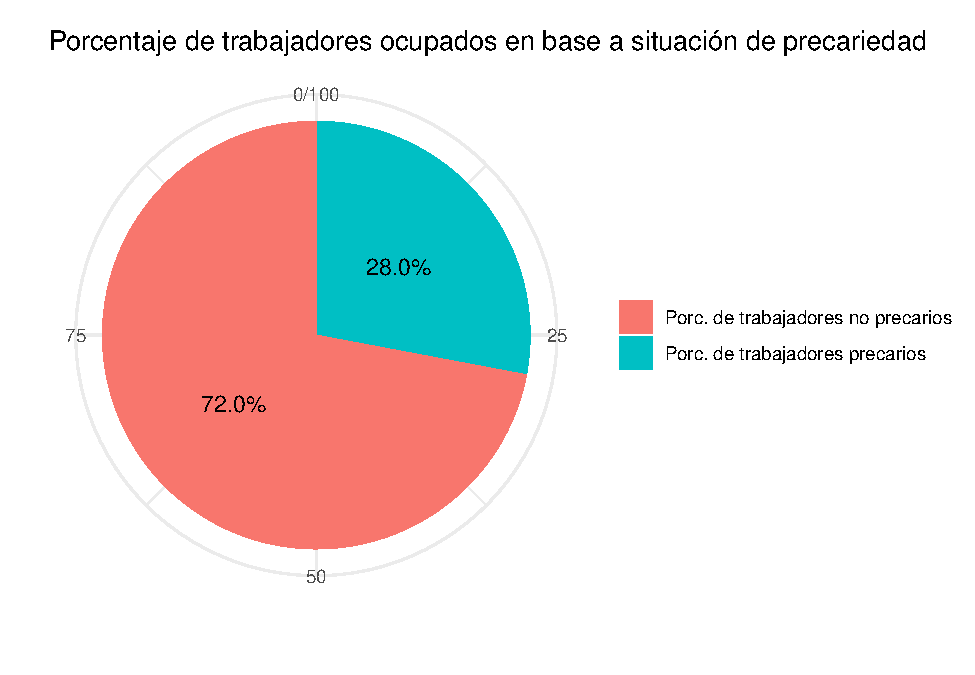
\includegraphics{TF_ASET_R_files/figure-latex/unnamed-chunk-9-1.pdf}

\subsection{Precariedad según sexo}\label{precariedad-seguxfan-sexo}

\begin{longtable}[t]{>{}c>{}c>{}c>{}c}
\caption{\label{tab:unnamed-chunk-10}Cantidad de trabajadores ocupados en base a la situación de precariedad}\\
\toprule
Sexo & Trabajador en precariedad & Trabajador en no precariedad & Población ocupada\\
\midrule
\cellcolor{white}{\textcolor{black}{\textbf{Hombre}}} & \cellcolor{white}{\textcolor{black}{\textbf{1.942.853}}} & \cellcolor{white}{\textcolor{black}{\textbf{5.535.230}}} & \cellcolor{white}{\textcolor{black}{\textbf{7.478.083}}}\\
\cellcolor{white}{\textcolor{black}{\textbf{Mujer}}} & \cellcolor{white}{\textcolor{black}{\textbf{1.795.861}}} & \cellcolor{white}{\textcolor{black}{\textbf{4.094.096}}} & \cellcolor{white}{\textcolor{black}{\textbf{5.889.957}}}\\
\bottomrule
\end{longtable}

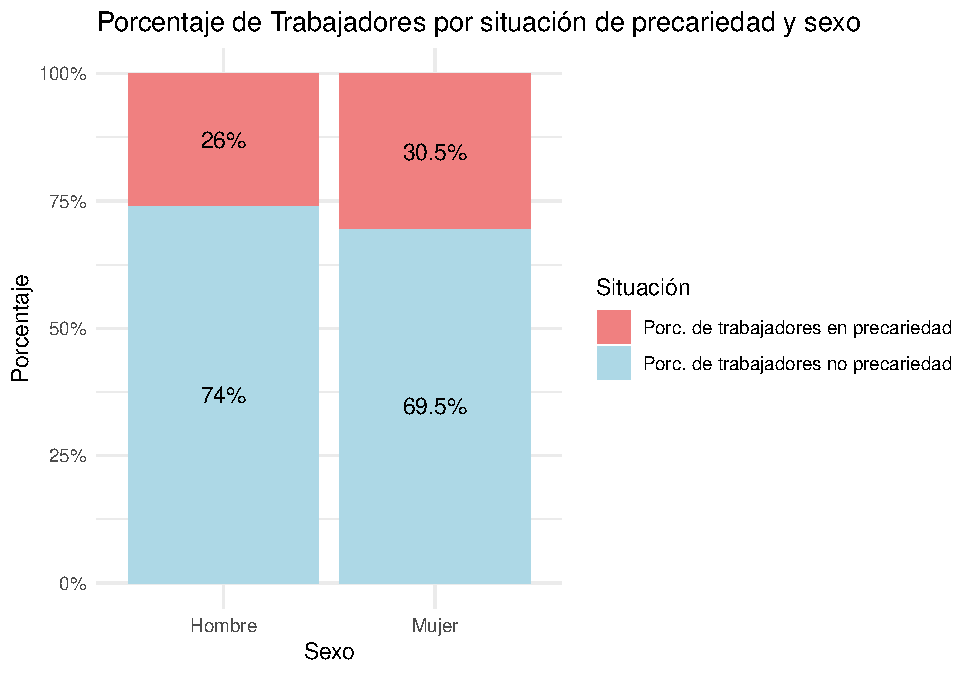
\includegraphics{TF_ASET_R_files/figure-latex/unnamed-chunk-12-1.pdf}

\subsection{Precariedad según franja
etaria}\label{precariedad-seguxfan-franja-etaria}

\begin{longtable}[t]{>{}c>{}c>{}c>{}c}
\caption{\label{tab:unnamed-chunk-13}Cantidad de trabajadores ocupados en base a la situación de precariedad y la franja etaria}\\
\toprule
Franja Etaria & Trabajador en precariedad & Trabajador en no precariedad & Población ocupada\\
\midrule
\cellcolor{white}{\textcolor{black}{\textbf{Adultos}}} & \cellcolor{white}{\textcolor{black}{\textbf{2.240.835}}} & \cellcolor{white}{\textcolor{black}{\textbf{7.589.603}}} & \cellcolor{white}{\textcolor{black}{\textbf{9.830.438}}}\\
\cellcolor{white}{\textcolor{black}{\textbf{Jov.15-18}}} & \cellcolor{white}{\textcolor{black}{\textbf{108.346}}} & \cellcolor{white}{\textcolor{black}{\textbf{34.692}}} & \cellcolor{white}{\textcolor{black}{\textbf{143.038}}}\\
\cellcolor{white}{\textcolor{black}{\textbf{Jov.19-24}}} & \cellcolor{white}{\textcolor{black}{\textbf{699.646}}} & \cellcolor{white}{\textcolor{black}{\textbf{550.774}}} & \cellcolor{white}{\textcolor{black}{\textbf{1.250.420}}}\\
\cellcolor{white}{\textcolor{black}{\textbf{Jov.25-29}}} & \cellcolor{white}{\textcolor{black}{\textbf{563.396}}} & \cellcolor{white}{\textcolor{black}{\textbf{985.115}}} & \cellcolor{white}{\textcolor{black}{\textbf{1.548.511}}}\\
\bottomrule
\end{longtable}

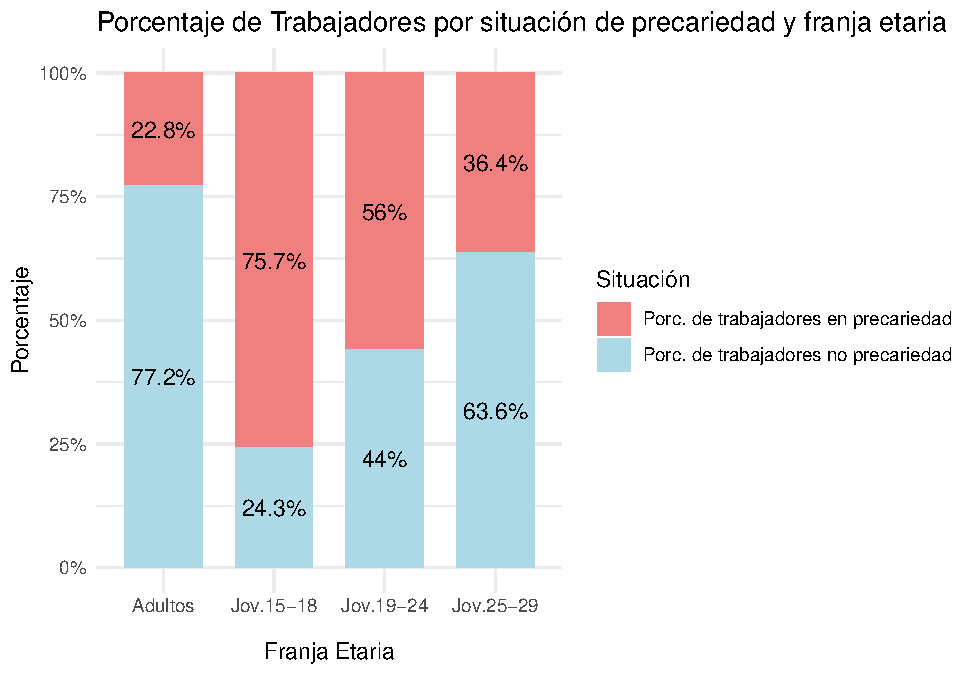
\includegraphics{TF_ASET_R_files/figure-latex/unnamed-chunk-15-1.pdf}

\subsection{Precariedad según nivel
educativo}\label{precariedad-seguxfan-nivel-educativo}

\begin{longtable}[t]{>{}c>{}c>{}c>{}c}
\caption{\label{tab:unnamed-chunk-16}Cantidad de trabajadores ocupados en base a la situación de precariedad y el nivel educativo}\\
\toprule
Nivel Educativo & Trabajador en precariedad & Trabajador en no precariedad & Población ocupada\\
\midrule
\cellcolor{white}{\textcolor{black}{\textbf{Menor a Secundaria}}} & \cellcolor{white}{\textcolor{black}{\textbf{1.514.579}}} & \cellcolor{white}{\textcolor{black}{\textbf{2.277.742}}} & \cellcolor{white}{\textcolor{black}{\textbf{3.792.321}}}\\
\cellcolor{white}{\textcolor{black}{\textbf{Secundaria Completa}}} & \cellcolor{white}{\textcolor{black}{\textbf{1.768.492}}} & \cellcolor{white}{\textcolor{black}{\textbf{4.259.158}}} & \cellcolor{white}{\textcolor{black}{\textbf{6.027.650}}}\\
\cellcolor{white}{\textcolor{black}{\textbf{Superior Completo}}} & \cellcolor{white}{\textcolor{black}{\textbf{455.643}}} & \cellcolor{white}{\textcolor{black}{\textbf{3.092.426}}} & \cellcolor{white}{\textcolor{black}{\textbf{3.548.069}}}\\
\bottomrule
\end{longtable}

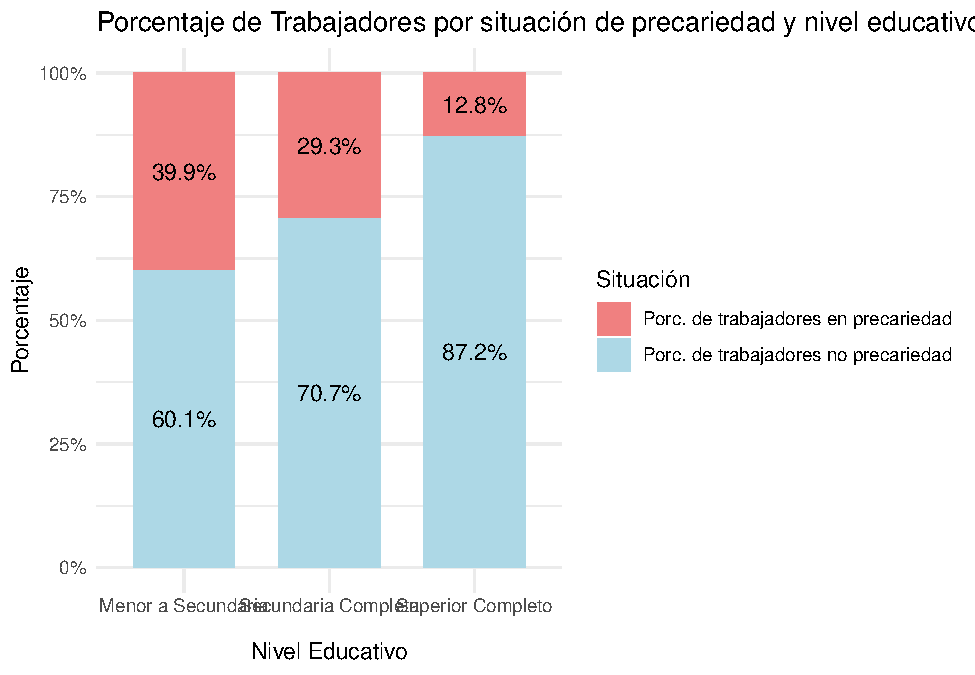
\includegraphics{TF_ASET_R_files/figure-latex/unnamed-chunk-18-1.pdf}

\end{document}
